\chapter{Introduction}
\label{chapter:intro}

\section{Cryptography}

Cryptography is the mathematical science of protecting secret information by transforming it into a form which is illegible. Generally, the original information is called \textit{plaintext} while the transformed information is called \textit{ciphertext}. Once plaintext is transformed into ciphertext, the latter can then be sent over an insecure channel to its destination. At the destination, the reverse transformation takes place yielding back the original information. Transformation of plaintext to ciphertext is referred to as \textit{encryption}, while the reverse process is called \textit{decryption}. A secret information called \textit{key} is used in both encryption and decryption. 

This cryptographic key can be compared with the key for locks which are used to provide safety of personal belongings. If the key is lost, then the lock can be opened by the holder of the key and our personal belongings can be stolen. Similarly, if an attacker knows the cryptographic key he can know the plaintext by decrypting the ciphertext, thus gaining knowledge of information supposed to be secret.  

This is just one application of cryptography in modern security systems, namely providing confidentiality to secret information; though it was this application with which the idea of cryptography was first conceived. Modern cryptography is also capable of providing message integrity (that a message has not been modified), authentication between two parties (the guarantee that we are talking with the expected party), non-repudiation (that a party cannot deny the fact that it has carried through a transaction, if it has really done so) and so on. 

In the late 19th century, Kerckhoff published a very important principle \cite{kerckhoff} which has become the basis of modern security systems using cryptography. He said that the security of a cryptographic encryption-decryption algorithm must rest solely in the secrecy of its key, not in the secrecy of the algorithm itself. In other words, while designing a security system with cryptography, all cryptographic algorithms must be openly published, while the only secret parameter should be the key used by the algorithm. This helps in the cryptanalysis of the algorithms and weaknesses can be found out by researchers and cryptanalysts. But more importantly, management of keys is much easier than management of algorithms as keys are small and algorithms are bulky.

Though this is a very important principle, still the design of security systems continue to be based on proprietary algorithms. More information on certain secret algorithms and successful reverse-engineering techniques is provided in section \ref{sec:hitag2-background}.

Two kinds of cryptosystems exist, depending on the manner in which keys are used: symmetric-key and asymmetric-key. In symmetric-key cryptography, a single key is shared between two communicating parties, such that one party encrypts plaintext using the shared key and the other party decrypts the received ciphertext using the same key. In such systems, the secrecy of the shared key becomes extremely critical. Also, if the number of parties grows, the number of keys required in the system becomes large, since each communicating pair would hold a different key. In addition, sharing keys between each pair requires secure key establishment protocols. 

Symmetric-key cryptography was the only known kind of encryption until Diffie and Hellman introduced the concept of asymmetric-key cryptography \cite{diffie1976ndc} for the first time in 1976. In asymmetric-key cryptography, the encryption and corresponding decryption are performed with different keys. Every party holds two keys: one public and one private. If \emph{Alice} wants to send a message to \emph{Bob}, she will encrypt the plaintext with the public key of \emph{Bob}. At the other end, \emph{Bob} would decrypt this ciphertext using his private key. The public-private key pair are related, but it is unfeasible to determine \emph{Bob}'s private key from his public key. Since every party holds two keys, the total number of keys is reduced considerably when compared to symmetric-key cryptosystems. Also, no key establishment protocols are needed as the public keys are distributed through public channels.

Symmetric-key algorithms are further classified into two different types, based on the manner in which plaintext is used by the encryption algorithm. These are block ciphers and stream ciphers. Block ciphers divide the plaintext into blocks of data, and each block is then encrypted separately. The sizes of the input and output blocks are same, irrespective of the size of the key. Successive output blocks are then connected to each other in some way, depending on the mode of operation of the block cipher. \emph{DES} (data encryption standard) has been one of the most widely used block ciphers with block size of 64 bits and key size of 56 bits. \emph{DES} has been recently replaced by \emph{AES} (advanced encryption standard) as the approved standard by NIST \footnote{http://www.nist.gov/}, through a public competition \cite{aes-process-wiki} which called for new block cipher designs to replace \emph{DES}.

Stream ciphers on the other hand, have a different functional structure and working. Stream ciphers consist of an internal state, which is used in deriving one output bit through an output function. The internal state changes over successive clock cycles using an update function, consequently producing a stream of bits at the output. The plaintext bits are then \emph{xor}'ed bit by bit with the output bits of the stream cipher to produce the ciphertext bits. The working of stream ciphers is explained in much detail in section \ref{sec:stream-cipher}. 

\section{Stream cipher}
\label{sec:stream-cipher}

\subsection{One-time pads} 
\label{sec:one-time-pads}

Before we explain the working of stream ciphers, it is important that we understand the motivation for the design of stream ciphers. An inspiration behind practical stream ciphers of today has been the one-time pad, which is also known as the Vernam cipher. In the one-time pad, the length of the key is required to be equal to or greater than the length of the plaintext. Each plaintext bit is operated with the corresponding key bit using the \emph{exclusive-or} (or \emph{xor}) operation, thus resulting in one bit of the ciphertext. So, if $p_i$ represents the $i^{th}$ bit of the plaintext, and $k_i$ represents the $i^{th}$ bit of the key, then the $i^{th}$ bit of the ciphertext is given by $c_i$ = $p_i \oplus k_i$ \cite{stamp2007acb}. The corresponding decryption takes place as $p_i$ = $c_i \oplus k_i$. This is shown in the figure \ref{fig:one-time-pad}.

\begin{figure}[ht!]
	\centering
		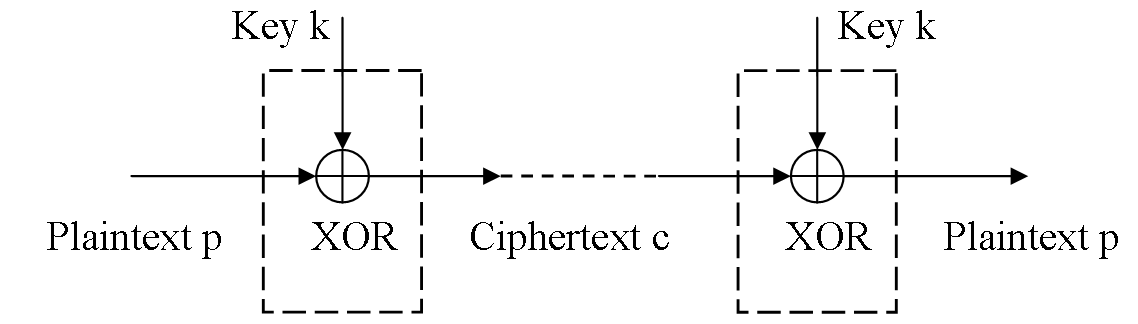
\includegraphics[width=4.4in]{./figures/one-time-pad.PNG}
	\caption{One-time pads}	
	\label{fig:one-time-pad}
\end{figure}

The key bits are required to be completely random, without any statistical correlation between them. With this pre-condition, there is no way that an adversary could determine the secret key just by knowing the ciphertext. Since the key bits are derived from a truly random source, there could be several combinations of the plaintext and the key which result in the given ciphertext. The attacker would, in such a scenario, never be able to determine which of the specific combination is the right one, even with infinite computing power at hand \cite{one-time-pads-link}.

If the attacker knows certain bits of the plaintext, then the corresponding bits of the key can be determined. If the key is not truly random, the attacker can predict some of the remaining bits of the key and thus decipher the remaining plaintext. Hence, the key should be truly random. 

Shannon in 1949, used his notion of information theory to formally prove that one-time pads are unbreakable \cite{shannon1949cts}, and termed them as having perfect secrecy. But for practical purposes, one-time pads have several weaknesses. These are explained in the following two points.
\begin{itemize}
\item The length of the key has to be equal to the length of the plaintext so that all the plaintext bits are encrypted. Thus to encrypt a long plaintext, large number of `random' key bits need to be generated. Managing such a huge set of key bits is not practical, since the storage and transfer need to be carried out securely. 

\item As the name of one-time pad suggests, a key can be used for just one transaction. If the same key is used for encrypting two different plaintext messages, the chances that the key being broken are extremely high. These chances are precisely zero when the key is used just for one encryption and is derived from a true random source. So it is suggested that a previous key not be used again.
\end{itemize}

Taking into consideration the weaknesses of one-time pads, it rather makes more sense to transmit the plaintext itself through the secure channel, than transmitting the key. Clearly, one-time pads are not good enough for being deployed in practical systems, but they reveal a strong design basis for stream ciphers. The component missing between one-time pads and stream ciphers is the pseudo-random sequence generator, which is discussed next. 

\subsection{Pseudo-random sequence generators}
\label{sec:psrg}

The only source of generating true random bits is through physical phenomena such as the rate of radioactive decay of an element or the thermal noise of a semiconductor diode \cite{goldberg1996ran}, which requires dedicated hardware device. If such device is not available, then computer programs are used to generate pseudo-random bits. These bits cannot be truly random as the computer is a finite state machine, and hence called pseudo-random.

Pseudo-random sequence generator (PRSG) is used to derive a seemingly random sequence of bits called the \emph{keystream}, using a small initial seed value. PRSG's are finite state machines having an internal state, which is initialized using the secret key, along with some more initialization parameters if required. A PRSG uses the following two functions internally.
\begin{itemize}
\item A linear \emph{update function} is used to derive the next state using the current state.
\item A linear or non-linear \emph{output function} is used to generate an output bit from the current state. 
\end{itemize}

\begin{figure}[ht!]
	\centering
		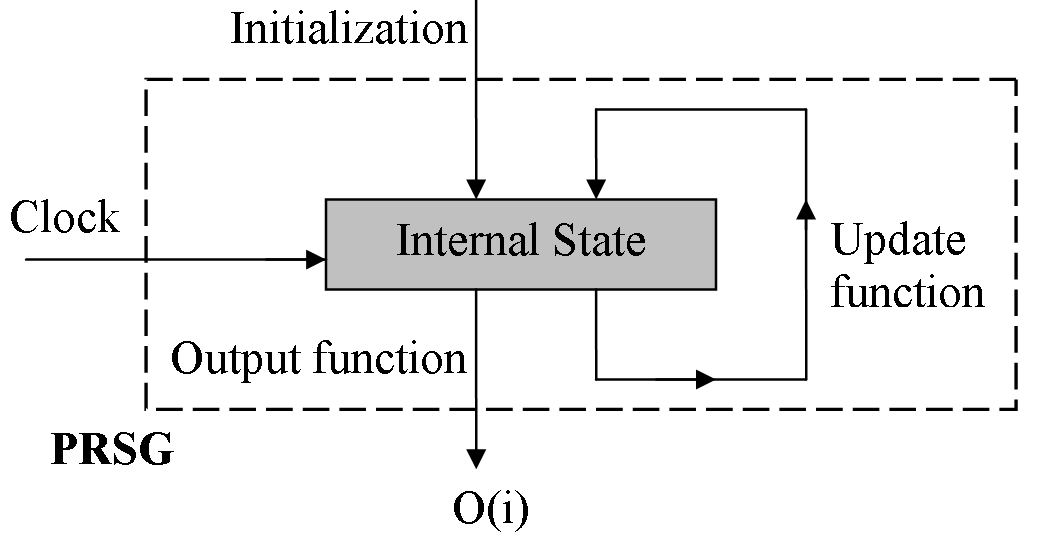
\includegraphics[width=3.5in]{./figures/prsg.PNG}
	\caption{Internal model of pseudo-random sequence generator}	
	\label{fig:prsg}
\end{figure}

Figure \ref{fig:prsg} shows the internal model of a PRSG. The clock signal is used to trigger a change of the internal state using the update function. Once the internal state changes, a new output bit is computed through the output function. A stream of such output bits (over several clock cycles) constitutes the keystream.

\paragraph{\textit{Use in stream cipher construction.}}
\label{para:stream-construction} 
In the construction of stream ciphers, we need to use secret keys of length which is fixed and independent of the length of plaintext. The secret key is used in the initialization of the PRSG thus generating a long keystream which replaces the long secret key of the one-time pads. The trade-off here is that the keystream is not truly random. As a result, the perfect secrecy of one-time pads does not apply to stream ciphers, but at the same time, the strength of the pseudo-random sequence generator becomes extremely important in determining how strong the stream cipher is cryptographically.

An overview of a stream cipher design is shown in figure \ref{fig:stream-cipher}. The secret key and other initialization parameters like initialization vector (IV) etc. are used to initialize the internal state. Once the initial state is prepared, the PRSG is ready to generate the keystream. Bits of the plaintext are \emph{xor}'ed along with corresponding bits from the keystream to generate a stream of encrypted bits. In effect, the plaintext and the keystream are used to produce the ciphertext.

\begin{figure}[ht!]
	\centering
		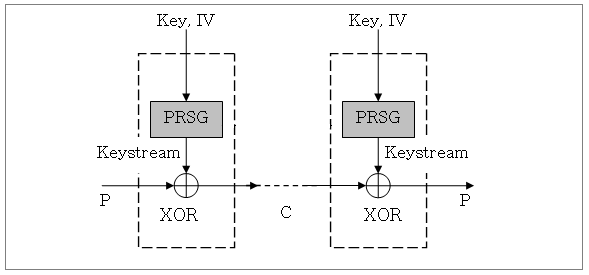
\includegraphics[width=3in]{./figures/stream-cipher.PNG}
	\caption{Deployment of PRSG in a stream cipher}	
	\label{fig:stream-cipher}
\end{figure}

At the receiver end, the PRSG is initialized using the same parameters. Any change in the initialization results in the generation of a different keystream leading to incorrect decryption of the received ciphertext. With the correct keystream, ciphertext is decrypted giving the correct plaintext. 

As briefly mentioned before, the security of the stream cipher much depends on the security properties of PRSG. The output sequence is required to behave as a true random sequence. One very important consideration in ascertaining adequate security \cite{robshaw1995sct} is mentioned below.

The period of the keystream should be large. This becomes extremely important when the length of the plaintext is large. If the keystream repeats, the same sequence would encrypt different parts of the plaintext. If the attacker has knowledge of some initial part of the plaintext, then the initial keystream encrypting the known plaintext can be recovered. This initial keystream can later be used to decrypt part of the ciphertext which the attacker does not know. Even if the attacker has no knowledge of plaintext, certain properties of the plaintext can be derived from the two ciphertexts encrypted using the same keystream. 

On the other hand, the requirement on how large the period should be depends on the amount plaintext expected to be encrypted.

\subsection{Linear feedback shift registers} 
\label{sec:lfsr}
The most widespread implementation of PRSG's is done using a linear feedback shift register (LFSR). Other methods for generating pseudo-random sequences exist as well. Since we are mainly going to deal with an LFSR based generator in this thesis (HiTag2, described in section \ref{sec:hitag2-cipher-description}), we would only describe them here. Other methods of generating pseudo-random sequences are linear congruence generators and non-linear feedback shift registers. For an introduction to these methods, we point to \cite{zeng1991pbg}. 
% reason why LFSR are widely used, and why are we more interested in them %
% more info on other generators %

It is important to note that LFSR constitutes only the \emph{update function} of the PRSG. The \emph{output function} of the PRSG needs to be implemented on top of the LFSR. An LFSR consists of two important components which are a shift register and a linear feedback function.\\

\noindent \textbf{\emph{Shift Register.}} A shift register holds a fixed number of bits, and shifts each of them into corresponding adjacent positions (all in a particular direction) on every clock cycle. If the direction of the shift is taken to be rightwards, then in every clock cycle there is a new bit on the leftmost position of the register, and the rightmost bit is excluded from the register, as shown in the figure \ref{fig:shift-register}. If the $n$ bits of the shift register are represented by $s_{n-1}$, $s_{n-2}$, $\ldots$ , $s_{1}$, $s_{0}$, then on every clock cycle we have the following transformations: $s_{out}$ = $s_{0}$, $s_{0}$ = $s_{1}$, $\ldots$ , $s_{n-2}$ = $s_{n-1}$, $s_{n-1}$ = $s_{in}$; where $s_{out}$ is the bit which is excluded from the register and $s_{in}$ is the new bit. The application implementing the shift register decides how the $s_{in}$ and $s_{out}$ bits are handled.

\begin{figure}[ht!]
	\centering
		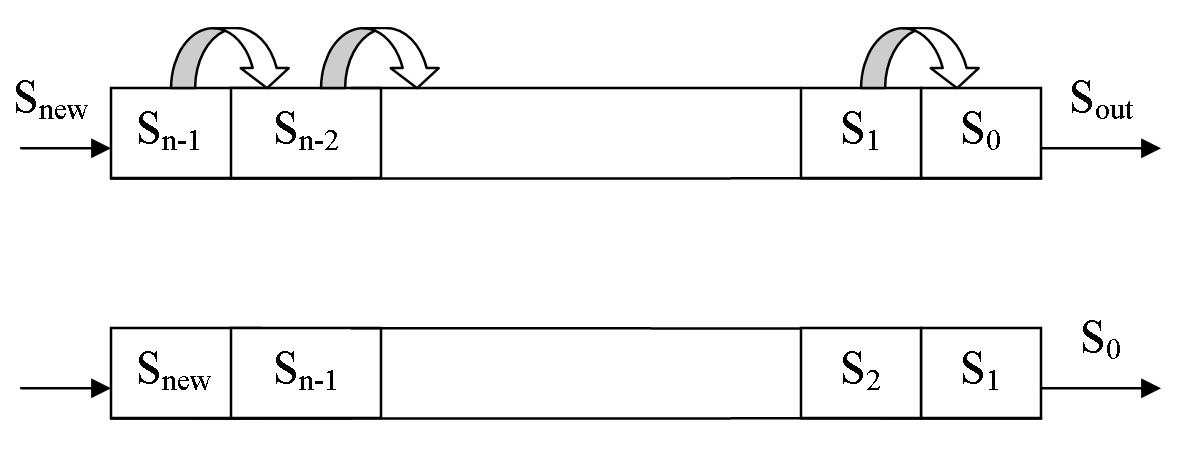
\includegraphics[width=4in]{./figures/shift-register.PNG}
	\caption{A simple shift register and its state after one clock cycle}	
	\label{fig:shift-register}
\end{figure}

For example, one of the uses of shift registers has been in the conversion of sequential (or serial) data to parallel data, and vice versa \cite{lfsr-link}. A sequence of bits can be stored in the shift register over a period of $n$ clock cycles, and retrieved in a parallel form in the $(n+1)$'th clock cycle. Hence, $s_{in}$ bit is taken from the input sequential stream, while $s_{out}$ bit is not used. 

For parallel-to-sequential data conversion, a parallel stream of $n$ bits is stored in the shift register in one cycle, and retrieved sequentially over the next $n$ clock cycles. The bit $s_{in}$ is not used in this case and $s_{out}$ stores bits of the sequential output stream.\\

\noindent \textbf{\emph{Linear feedback.}} A \textit{feedback function} defines the $s_{in}$ bit as a function of one or more bits from among the $n$ bits of the shift register. If the function is \textit{linear}, it said to be a \textit{linear feedback function}. Linearity is incorporated in the design generally by the use of $xor$ as the feedback function. Other boolean functions which are linear are negation, logical biconditional, tautology, and contradiction. According to the Wikipedia page on linearity \cite{linear-wiki}, 
\begin{quote}
\footnotesize{A Boolean function is linear if (1) In every row of the truth table in which the value of the function is `T', there are an even number of `T's assigned to the arguments of the function; and in every row in which the truth value of the function is `F', there are an odd number of `T's assigned to arguments; or (2) In every row in which the truth value of the function is `T', there are an odd number of `T's assigned to the arguments and in every row in which the function is `F' there is an even number of `T's assigned to arguments.
}
\end{quote}

The above properties can be easily checked to hold in the truth table of the \emph{xor} function.

A simple example of an LFSR is shown in figure \ref{fig:lfsr-example1}. Let us examine the linear feedback function more closely for this example. As can be seen, certain selected bits from the shift register are \emph{xor}'ed, and the resulting value is assigned to the leftmost bit (but only in the next clock cycle) in addition to the shifting of bits. As a result, the internal state of the LFSR is changed. If we number the bits from \emph{1, 2,} $\ldots$ , and so on, then the bits 11, 13, 14 and 16 are used in the feedback function. These bits are referred to as \emph{tap sequence} or $taps$ of the LFSR. In general, the outputs that affect the input of the LFSR are called $taps$.\\


\begin{figure}[ht!]
	\centering
		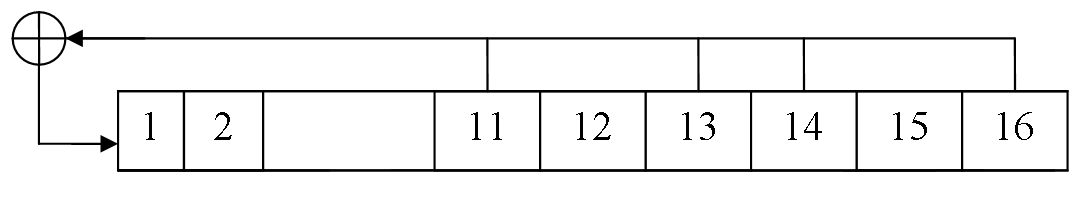
\includegraphics[width=4in]{./figures/lfsr-example.PNG}
	\caption{A simple LFSR of size 16 bits and tap bits 11, 13, 14 and 16}	
	\label{fig:lfsr-example1}
\end{figure}

\noindent \textit{\textbf{Maximal length tap sequence.}} Depending on the initial state, the LFSR runs through a set of states and then returns back to the initial state. This forms a cycle of states. In order to use the LFSR for generating a pseudo-random sequence, we want to have the longest cycle of the LFSR states. In other words, we want the LFSR to traverse through all possible states, which is equal to $2^n$, where $n$ is the number of bits in the shift register. 
%This is important since it is desired that the pseudo-random sequence has a large period, as mentioned in the requirements for PSRG in section \ref{para:stream-construction}.

It is important to note that if the LFSR is in a state where all the bits are 0, then the next state would also be the same. This condition occurs because the \textit{xor} of any number of 0's is always 0. Such a state is called the \textit{trivial state}. As a result, no cycle is formed if the LFSR is initialized with the trivial state. Hence on excluding the trivial state, the number of different states in the LFSR forming a cycle becomes $2^n-1$. A tap sequence which generates this particular cycle of states is called the \textit{maximal length tap sequence}. 

Moreover, from \cite{erik-discussions}, nothing can be said about the period of the keystream if the period of the LFSR is $2^n-1$. This is so because the keystream not only depends on the internal state, but also on the output function. If a weak output function is chosen, the keystream can start repeating before the LFSR states repeat. Much depends on the linearity of the output function.

The tap sequence for the LFSR in figure \ref{fig:lfsr-example1} is a maximal length tap sequence. A tap sequence can be verified to be a maximal length by analyzing the polynomial representation of the tap sequence.\\

\noindent \textit{\textbf{Polynomial representation of tap sequence.}} Once we have a tap sequence, we can express it in the form of a polynomial with modular \textbf{2} coefficients. For the example shown in figure \ref{fig:lfsr-example1}, the polynomial representation of the tap sequence is

\begin{center}
$p(x)$ =  1 + $x^{11}$ + $x^{13}$ + $x^{14}$ + $x^{16}$
\end{center}

The powers of $x$ represent the tap bits. The 1 in the starting is a result of $x^0$ and represents the $s_{in}$ bit, since $s_{in}$ can be interpreted to exist at the 0'th position of the shift register (theoretically). A given tap sequence is a maximal length tap sequence if the polynomial representing it is irreducible i.e.~the polynomial cannot be factored into nontrivial polynomials.

It is important to note that the polynomial representation should not depend on the numbering of the bit positions. If the same LFSR is numbered in the fashion as shown in figure \ref{fig:lfsr-example2}, then we have the following polynomial representation.
\begin{align*}
p'(x) &= x^{17} + x^{6} + x^{4} + x^{3} + x
\end{align*}
\begin{align}
\label{eq:poly-1} p'(x) &= x*(x^{16} + x^{5} + x^{3} + x^{2} + 1)\\
\label{eq:poly-2} p'(x) &= x^{16} + x^{5} + x^{3} + x^{2} + 1
\end{align}

\begin{figure}[ht!]
	\centering
		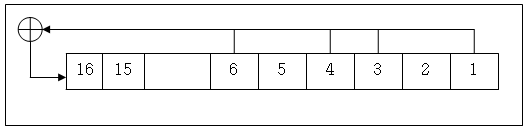
\includegraphics[width=4in]{./figures/lfsr-example-reverse.PNG}
	\caption{A different numbering of the bit positions for the same LFSR}	
	\label{fig:lfsr-example2}
\end{figure}

The polynomial in equation \ref{eq:poly-1} is irreducible only if the term $(x^{16} + x^{5} + x^{3} + x^{2} + 1)$ is irreducible, so we rewrite $p'(x)$ in equation \ref{eq:poly-2} after ignoring the factor $x$. Since both $p'(x)$ and $p(x)$ represent the same LFSR, they should be related in some way. The Wikipedia page for LFSR at \cite{lfsr-wiki} states the following in this context,

\begin{quote}
\footnotesize{
Once one maximal tap sequence has been found, another automatically follows. If the tap sequence, in an $n$ bit LFSR, is [n,A,B,C,0], where the \textbf{0} corresponds to the $x^0$ = 1 term, then the corresponding `mirror' sequence is [n,n-C,n-B,n-A,0].}
\end{quote}

In our example, the tap sequence [16,14,13,11,0] has a mirror tap sequence [16,5,3,2,0], which are represented by the polynomials $p(x)$ and $p'(x)$.

The bottom line is this: the choice of an appropriate polynomial for the LFSR is important so as to guarantee that the LFSR moves through the cycle of $2^n-1$ states. This polynomial should have the property of being irreducible.

\section{The HiTag2 stream cipher}
\label{sec:hitag2}

\subsection{Background}
\label{sec:hitag2-background}
HiTag2 is a stream cipher originally designed by Philips Semiconductors (now NXP Semiconductors) and used for mutual authentication between a car remote control and controller in the car. Such systems (called remote keyless entry or RKE systems) have been widely implemented in modern electronic cars, and facilitate locking and unlocking of car doors upon just a button press from within a certain maximum distance from the car \cite{rke-wiki}. The system designed by NXP in addition to RKE, also incorporates vehicle immobilizer which prevents ignition of the engine if someone breaks into the car. Only the correct car key which uses the secret digital key can authenticate itself to the car controller, thus allowing the ignition \cite{rke-nxp}.

The HiTag2 stream cipher provides two-way authentication, authenticating the two entities to each other one by one. In such a protocol, a nonce is sent across from the initiator to the responder. The responder initializes the stream cipher using the nonce as IV, additionally using the secret key and its fixed ID. Some fixed length of the keystream is then sent back to the initiator as authenticator. The similar protocol is executed to authenticate the initiator to the responder. 

But, this is just one use of the cipher, and other applications could use the cipher for authentication as well as encryption. If secrecy of the plaintext is desired, the message bits are \emph{xor}'ed with the keystream bits before sending them over the public channel. 

HiTag2 was kept secret by Philips until it was reverse-engineered using the cipher's software implementation. The microcode (or assembly code) of HiTag2 was decompiled from the implementation available in the car remote controls and the RKE receivers. The C code for the cipher is available on the website \cite{hitag2-code}. A full system level specification of the RKE system by Philips (titled Active Tag and IC) which implements the HiTag2 cipher is also available \cite{active-tag-datasheet}. HiTag2 now is the intellectual property of NXP, but the specification document holds the name of Philips since NXP did not come into existence at that time in 2005. Also, since the cryptography (HiTag2) on the RKE system was kept secret at that time, HiTag2 modes are just mentioned without any further information on the functional working of the cipher.

The design of HiTag2 is very similar to a recently reverse-engineered \cite{NohlESP-2008-usenix} stream cipher called Crypto-1, which is used in Mifare Classic smartcards by NXP. The Mifare family comprises of contactless smart cards and card readers, with a variety of different features including availability of memory on the cards to store data with read/write permissions on the cards. As a result of these features, Mifare system is widely used in applications requiring more than just authentication. Some such applications are ticketing system for public transportation (OV-Chipkaart in Netherlands, Oyster cards in UK etc.) and access control in buildings. Crypto-1 cipher used in Mifare Classic cards and readers was kept secret until recently Nohl et al.~\cite{NohlESP-2008-usenix} reverse-engineered the algorithm from its silicon implementation.

In addition, the same Mifare Classic cards and readers are shown to be easily clonable \cite{dekoninggans2008pam} by researchers at Radboud University. They have analyzed the communication protocol between the card and the reader, and have been been able to show that there are several weaknesses in the Crypto-1 cipher. They have been able to recover the necessary keystream by analyzing the protocol messages. The details of this protocol analysis complements the work by Nohl et al., and using both the ideas, mounting brute-force attack on the cipher has been made possible. 

Apart from reverse-engineering from software or hardware implementations, a black-box reverse-engineering has also been applied to break secret algorithms. The DST RFID tag (using the DST stream cipher) was broken in 2005 using black-box reverse-engineering \cite{bono2005sac}, i.e.~by selecting certain input formats and using both the input and output combinations to deduce the structure and working of the cipher. The most common application of Texas Instrument's DST tag is in vehicle immobilizer systems and electronic payment systems \cite{dst-rfid-analysis}. 

In the next section, the working of HiTag2 is described.

\subsection{Cipher description}
\label{sec:hitag2-cipher-description}
The basic components of the HiTag2 stream cipher are outlined below.
\begin{itemize}
\item 48 bit key
\item 32 bit serial ID
\item 32 bit initialization vector (IV)
\item 48 bit internal state with linear update function (basically, an LFSR)
\item Non-linear output function based on multiplexor, with data bits being constant and address bits depending on the current internal state
\end{itemize}

The entire setup of the keystream generator is done in two phases. The first phase is the initialization of the LFSR, which sets the internal state to a non-zero value using the key and the serial ID. The second phase is the setup of the LFSR during which the LFSR is clocked (resulting in the shifting of bits) using the key and IV bits in the process. Once the LFSR is set, the keystream is ready to be generated from the internal state right away. We describe these phases in detail here.\\ 

\noindent \textit{\textbf{1. LFSR Initialization.}} The initialization step of the LFSR is straightforward. Instead of initializing the LFSR with random bits, the serial ID and an initial part of the key are used. The 32 bits of the serial ID are stored in the least significant 32 bits of the LFSR (bits from index 0 through index 31). Then, the least significant 16 bits of the key are stored in the remaining 16 bits of the LFSR (bits from index 32 through index 47), as shown in figure \ref{fig:hitag2-1}. With this the initialization of the LFSR is complete.\\

\begin{figure}[ht!]
	\centering
		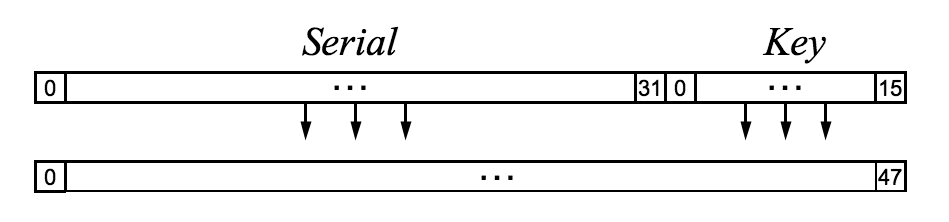
\includegraphics[width=4.3in]{./figures/hitag2-1.PNG}
	\caption{LFSR Initialization \cite{hitag2-figure}}	
	\label{fig:hitag2-1}
\end{figure}

\noindent \textit{\textbf{2. LFSR Setup.}} During the setup of the LFSR, the 32 bits of IV are used with the remaining 32 bits of the key. The bits in the LFSR are shifted to the right in every clock cycle, and a new value is stored in the leftmost bit. In every clock cycle, an xor of the following three bits is computed: one bit from the key (range: bits from index 16 through 47), one bit from the IV (range: bits from index 0 through 31) and the output bit from the non-linear output function. The computed bit is stored at the leftmost bit of the LFSR. After 32 clock cycles, the internal state is prepared for keystream generation. This is shown in figure \ref{fig:hitag2-2}.\\

\begin{figure}[ht!]
	\centering
		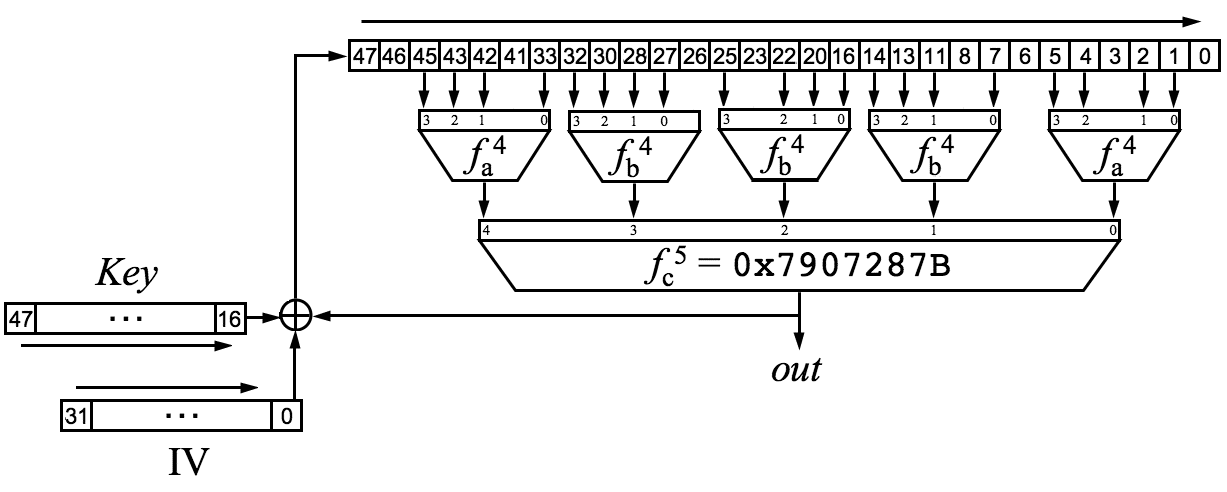
\includegraphics[width=5.5in]{./figures/hitag2-2.PNG}
	\caption{LFSR Setup Phase \cite{hitag2-figure}}	
	\label{fig:hitag2-2}
\end{figure}

\noindent \textit{\textbf{Output function.}} The output function consists of two levels of multiplexors. The multiplexors have fixed data bits, whereas the address bits are chosen either from the LFSR or from other multiplexors. In the first level, 20 bits from the LFSR are used as address bits to five four-bit multiplexors, giving a total of five bits of output (one from each multiplexor). These five bits are then used as address bits to the single five-bit multiplexor in the second level. The output of this multiplexor is the output bit of the stream cipher. In all, six instances of multiplexors cover the two levels of the output function.

\begin{table}[ht!]
\begin{center}
\small{
\begin{tabular}{|p{2.2cm}|l|p{2cm}|p{2.8cm}|p{1.5cm}|}
\hline 
\textbf{Multiplexor instance}	& \textbf{Function}		& \textbf{Data bits}	& \textbf{Address bits (input)}		& \textbf{Output bit}\\ \hline \hline
\multicolumn{5}{|c|}{Level 1 Multiplexors}\\ \hline \hline
MUX 1 			&	$f_a^4$			& 0x2C79			& 1, 2, 4, 5							& $o_1$\\
MUX 2 			&	$f_b^4$			& 0x6671			& 7, 11, 13, 14						& $o_2$\\
MUX 3 			&	$f_b^4$			& 0x6671			& 16, 20, 22, 25					& $o_3$\\
MUX 4 			&	$f_b^4$			& 0x6671			& 27, 28, 30, 32					& $o_4$\\
MUX 5 			&	$f_a^4$			& 0x2C79			& 33, 42, 43, 45					& $o_5$\\ \hline \hline
\multicolumn{5}{|c|}{Level 2 Multiplexor}\\ \hline \hline
MUX 6 			&	$f_c^5$			& 0x7907287B	& $o_1$, $o_2$, $o_3$, $o_4$, $o_5$		& \textit{out}\\ \hline
\end{tabular}}
\end{center}
\caption{Multiplexors making the output function in HiTag2}
\label{tab:muxs}
\end{table}

Three different multiplexor functions are used to realize these six instances, and these are called $f_a^4$, $f_b^4$ and $f_c^5$. While $f_a^4$ and $f_b^4$ take in four bits for addressing the output, $f_c^5$ takes in five bits. The multiplexors $f_a^4$ and $f_b^4$ are used in the first level, where as $f_c^5$ is used in the second level. These six instances are described in the table \ref{tab:muxs}. In the table, the input bits for the first level of multiplexors are indicated by the index of their position in the LFSR.

It is important to note that the update function of the LFSR is not used in both the initialization and setup phases of the cipher. This function is used during the keystream generation as discussed next.\\

\noindent \textit{\textbf{3. Keystream Generation.}} The output from the function $f_c^5$ constitutes the keystream. In addition, the LFSR state is changed in every clock cycle through the update function. The internal state is updated linearly, in the following fashion: the leftmost bit of the LFSR is replaced with the \textit{xor} of taps of the LFSR (which are bits 0, 2, 3, 6, 7, 8, 16, 22, 23, 26, 30, 41, 42, 43, 46 and 47). The remaining bits are shifted rightwards to adjacent positions. Once the internal state is changed, the output bit gets recomputed, generating the next bit of the keystream. This is shown in figure \ref{fig:hitag2-3}. 

\begin{figure}[ht!]
	\centering
		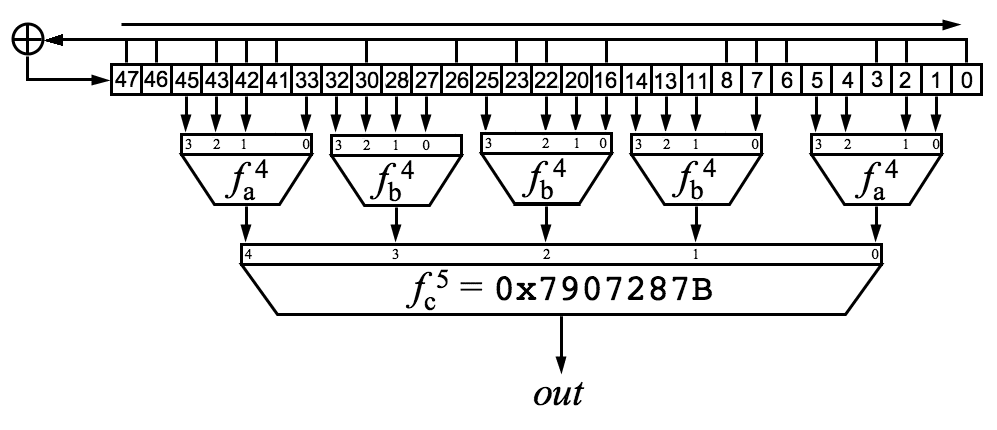
\includegraphics[width=4.3in]{./figures/hitag2-3.PNG}
	\caption{Keystream Generation \cite{hitag2-figure}}	
	\label{fig:hitag2-3}
\end{figure}

This completes a basic description of the cipher. 

A security critical aspect to consider here is the period of the HiTag2 LFSR. It is possible to check the period of the LFSR and ascertain if HiTag2 LFSR gives the maximal period of $(2^{48} - 1)$ or not. From previous discussion, the polynomial representation of the LFSR should represent an irreducible polynomial, if maximal period is to be achieved. We made an attempt to investigate this for HiTag2, but realized that huge computational time is required to do this. In order to check if the HiTag2 polynomial is irreducible, all the factors of the polynomial need to be checked. This takes time of the order of $2^{48}$, which could take months to complete on a dedicated personal computer.

We encoded the polynomial in Matlab, as shown in appendix \ref{app:irreducible-polynomial}. The program was run for a day without any decisive output. If the polynomial could be factorized by a small polynomial, the program would have shown the result and terminated; but this did not happen. Hence, we conclude that there are no small factors in the HiTag2 LFSR polynomial. On a more positive note, we believe that the polynomial is maximal, and we continue the rest of the thesis under this particular assumption.

The HiTag2 library is provided in appendix \ref{app:hitag2-lib}. We have taken the original implementation available at \cite{hitag2-code} and added certain functions to that. The functions that exist in the original code are mentioned below. 
\begin{itemize}
\item \textit{hitag2\_init}, performs setup and initialization of the internal state
\item \textit{f20}, gives the output bit from the internal state \footnote{This function has been renamed to \textit{hitag2\_output} in our implementation}
\item \textit{hitag2\_round}, gives the next output bit by updating the internal state and then calling the \textit{hitag2\_output} function
\item \textit{hitag2\_byte}, gives one byte of output with the most-significant bit representing the latest output bit
\end{itemize}

The following functions have been added to the original set of functions and assist in the tradeoff attacks. The names of these functions are: \textit{hitag2\_prefix}, \textit{hitag2\_prev\_state}, \textit{hitag2\_next\_state} and \textit{hitag2\_find\_key}. The relevance of these functions is explained in the next chapter. 

%\begin{itemize}
%\item \textit{hitag2\_prefix}, returns the prefix of the internal state; length of prefix is passed as parameter
%\item \textit{hitag2\_prev\_state}, gives the state occurring previous to the current state
%\item \textit{hitag2\_next\_state}, gives the state occurring next to the current state
%\item \textit{hitag2\_find\_key}, gives the key corresponding to the initial state
%\end{itemize}

\section{Time-memory tradeoff attack}
\label{sec:tmto-attack-intro}
\noindent \textit{\textbf{Brute force attack.}} A brute force attack on a block cipher would be to try out all the possible keys which could be used to encrypt certain known (or chosen) or unknown plaintext. The key which decrypts the ciphertext to give the known plaintext or most sensible plaintext (if it is unknown) is then the original key. Though very simple in theory, brute force attacks require a very long time to break ciphers in practice. There is no storage required during this attack, but the time required to break the cipher is very long. Though modern computers have advanced tremendously in their computational speed over the last some years, design of new ciphers have incorporated longer key sizes to protect against brute force attacks, rendering brute forcing still impractical.

For example, in order to break a 32 bit key, we would need to carry out $2^{32}$ decryptions on available ciphertext. Using a 2GHz processor (which is quite common for personal use), we can run $2^{31}$ clock cycles in one second (as 1 giga is $2^{30}$). Since one encryption would take a fixed number of clock cycles, say a modest $2^3$ cycles, by simple calculation, we can have a brute force attack on the cipher in $2^4$ seconds, or 16 seconds. As can be seen, this is a dismally weak key size. For a key size of 48 bits, the brute-force would take $2^{20}$ seconds which is 1048576 seconds, or just more than 12 days. In modern ciphers, the key sizes starting from 128 bits in length are considered safe. AES uses a minimum key size of 128 bits, which can be extended to use 256 bits. So, just to give a feeling of the security of a 128 bit cipher, it would take an order of $10^{30}$ years to brute force the key.\\

\noindent \textit{\textbf{Precomputed ciphertext attack.}} Brute-force attacks are just one side of the coin. The other way of breaking a cipher in a known (or chosen) plaintext attack is to precompute ciphertexts corresponding to all the possible keys and to store the (key, ciphertext) pair in a table in memory. During the attack, the attacker just needs to do a table lookup for the available ciphertext to find the corresponding key. Again, the concept is quite straightforward theoretically, but it also faces the same problem as brute-force attacks, but with a different parameter. A table lookup takes constant time (if efficient hash tables are implemented), so practically the attack time is very less. But, the size of precomputed data is tremendous and the attacker would need huge amount of memory to store this data for the attack phase. 

Let us again take the weaker case of a 32 bit key, which is far from use in today's ciphers. For each of $2^{32}$ possible keys, we need to store 32 bits of key and 32 bits of ciphertext (assuming the plaintext is 32 bits, which could very well be more). This amounts to 64 bits or 8 bytes of data for every possible key. $2^{32}$ such entries would require $2^{32} \times$ 8 bytes which is 32 gigabytes. For a random access memory, 32 GB is a high requirement. For higher key sizes, this requirement gets much away from practicality.\\

\noindent \textit{\textbf{In between time and memory.}} The technique of time-memory tradeoff or TMTO is a way between the above two extreme and practically difficult ideas. TMTO solves our problem by using memory in order to reduce the time for attack, bringing the requirements for time and memory within  practical domains. Before we go into more details of the working of time-memory tradeoff attacks on ciphers, we take a simple example of a general application of such tradeoffs. The example has been taken from \cite{stamp2003out}. \\

\noindent \textit{\textbf{Simple example.}} Consider the problem of finding the number of \textbf{1}'s in the binary representation of a non-negative integer $x$ (which takes $4$ bytes). The simplest algorithm to solve this problem would over 32 operations, pick the value of the least significant bit, add it to a variable \textit{sum} and shift $x$ rightwards by one bit. Variable \textit{sum} would then hold the desired result. The pseudo-code for such an algorithm is shown below.

\begin{lstlisting}[frame=tb]
/* ones_count(x) */
sum = 0
for i = 0 to len(x) - 1
    sum = sum + (x >> i) & 1
next i
return sum
\end{lstlisting}

Here, $>>$ denotes the right shift operation and \& denotes bitwise binary \emph{and} operation. The algorithm performs 32 operations (which is based on the length of the integer) and has nearly no memory requirement. The other approach to solve this problem would be to precompute and store the answer for each of the possible $2^{32}$ integers in memory. This way, just one memory lookup is required to find the result for $x$. But in this case, we need to have a memory of the order of $2^{32}$. 

One middle way between both these approaches would be to store the \textit{sum} for all possible 8 bit numbers, rather than doing it for all 32 bit numbers. Then the memory required would be of the order of $2^{8}$. To find the answer for $x$, we break the integer into blocks of 8 bits, and add the stored \textit{sum} for each of the blocks, by looking them up in the table. If $y_1$, $y_2$, $y_3$ and $y_4$ are the four blocks, such that

\begin{center}
$y_4$ = ($x$ $\&$ $0$xFF)\\
$y_3$ = ($(x >> 8)$ $\&$ $0$xFF)\\ 
$y_2$ = ($(x >> 16)$ $\&$ $0$xFF)\\ 
$y_1$ = ($(x >> 24)$ $\&$ $0$xFF)\\
\end{center}

and if p is the array which stores the \textit{sum} for all the 8 bit numbers, then the desired \textit{sum} for $x$ is calculated by

\begin{center}
$sum = p[y_1] + p[y_2] + p[y_3] + p[y_4]$\\
\end{center}

Four operations are performed in this case, as four lookups are made to the precomputed array $p$. This is just one way of realizing the time-memory tradeoff. If the algorithm stores 4 bit blocks, with their corresponding \textit{sum}, then the number of operations would be eight. Hence the optimal combination of memory and time can be chosen based on the resources at hand and the application. 

So, it is easy to see the advantage gained from tradeoff schemes as compared to schemes based on extreme requirements for time or memory. 

\section{Some important concepts}

In this section, we provide some building blocks which would be used throughout the thesis. We first introduce the idea of \textit{birthday paradox} and then introduce \textit{hashtables}.

\subsection{Birthday paradox}
\label{sec:bday-paradox}

\indent \textit{\textbf{General birthday paradox.}} Birthday paradox (or birthday problem or surprise, as it is also called), refers to the fact that in a room of 23 people, two people have the same date of birth with a probability greater than one-half. While there are 365 different possible birthdays in a year (excluding the leap year), the birthday paradox looks surprising and non-intuitive at the first glance. But, the figure has been derived from probability theory and is proved. 
% IMP: need a reference here %

A generalized definition of the birthday paradox for can be formulated as follows: given $n$ random integers where each could have $m$ different possible values, the probability that two of them would have the same value is given by the following equation \cite{menezes}.
\begin{center}
$P(m,n)$ $\approx$ $1 - e^{-{n^2}/{2m}}$
\end{center}
If we replace $m$ by 365, and $n$ by 23 in the above equation, then it can be checked that $P(365,23)$ $\approx$ $0.507$. In addition, $P(365,n)$ rapidly increases as $n$ increases, and the chances of two people having the same birthday becomes nearly $99 \%$ for $n$ = 57. If $m$ is considered to be very large, such that $m \rightarrow \infty$, then the above equation can be reduced for $P(m,n) \approx 1$, giving us the following condition. 
\begin{align}
\label{eq:birthday-paradox} n = \sqrt{\pi/2 \times m}
\end{align}

Equation \ref{eq:birthday-paradox} represents the condition for a set of $n$ numbers with $m$ different possible values to have two occurrences of a same number. This general birthday paradox is used in cryptography in determining collisions in hash functions. Consider a hash function $H$ with $h$ bits of output. The total number of different outputs the function could produce is $2^{h}$. A collision is said to occur when the hash function produces the same output for two different inputs, i.e.~$H(x_1)$ = $H(x_2)$ when $x_1$ $\neq$ $x_2$. Then, according to the birthday paradox, the chances that a collision would occur are close to $100 \%$ after the hash function has produced outputs for $2^{h/2}$ random inputs (if we have $m = 2^h$ and we ignore the factor of $\pi/2$).\\

\noindent \textit{\textbf{Variant of the birthday paradox.}} A variant of the birthday paradox (\cite{GeneralizedAttack}) is especially more interesting to us, since it is directly used in TMTO attacks. If we consider two groups of people now instead of one, then just 17 people are required to be present in each group, so that two people belonging to different groups share the same birthday.  

We can generalize the above situation in the following way. We have two groups of random elements each having different number of elements, say $n_1$ and $n_2$. The elements are non-negative integers, with both the groups having the same range $m$ for the integers. According to \cite{menezes}, the probability of at least one coincidence in such a case is given by,
\begin{center}
$P(m, n_1, n_2) = 1 -(1 - n_2/m)^{n_1}$
\end{center}
For the condition that $m \rightarrow \infty$, the above relation is reduced to,
\begin{center}
$P(m, n_1, n_2)$ $\approx$ $1 - e^{-{n_{1} n_{2}}/{m}}$
\end{center}
In order to find the condition for 100\% chances of a coincidence, we have $P(m, n_1, n_2) \approx 1$ and we take the limit $m \rightarrow \infty$ for the above equation. The following condition is then derived.
\begin{align}
\label{eq:n1-n2-m-condition} n_1 \times n_2 = \pi/4 \times m
\end{align}
If we replace $m$ by 365 and impose $n$ = $n_1$ = $n_2$, then we get $n$ = 16.93 $\approx$ 17. Hence, at least 17 people must be present in a room if the chances are 100\% that two people having the same birthday are present in both the groups. 

We further ignore the factor of $\pi/4$ in equation \ref{eq:n1-n2-m-condition} to get a simpler condition.  
\begin{align}
\label{eq:bday-paradox2} n_1 \times n_2 \geq m
\end{align}
Equation \ref{eq:bday-paradox2} is the birthday paradox we would use in the analysis of most of the tradeoff attacks on HiTag2.

% Add the case of handbook statement, with or without replacements?
% also briefly how this paradox would be applied to the TMTO?

% -------------
% what the simple birthday paradox is %

% generalize it in terms of n %

% introduce birthday attack, define scenario (then take hash as example) %

% what is the variant of birthday paradox %

% meet in the middle attack on DES by diffie hellman %
% a TMTO attack would always use variant of birthday attack %

% Question - How can the variant of the birthday problem be derived from the birthday problem?
% Question - Probability of one-half on 23, or is it one? root(pi * m / 2)
% Question - Is meet in the middle attack a TMTO attack? (I think NO!)
% --------------

\subsection{Hash tables}
\label{sec:hash-tables}


%Hash tables are used during the precomputation phase as a data structure to store the (prefix, state) pairs in memory. The advantage that hash tables %offer is in terms of the search time. The search time provided by hash tables in the best case and the average case is close to $O(1)$, while the %worst case search time is $O(n)$ occurring with very less probability. A very important role is played by the hash function chosen for the table. 

Hash tables are data structures designed with the purpose of searching through data in constant time. Consider a data structure $d$ in memory containing a huge set of elements stored one after the other. Given this data structure, we want to search an element $e$ in $d$. The only way to perform this action is to go through each element in $d$ and check if $e$ matches with that element. The number of operations in the worst case is equal to the number of elements in $d$. Hence, as $d$ increases, the worst case search time increases. A hashtable $h$ reduces the dependency of search time on the size of the data structure, and using $h$ as the data structure, $e$ can be searched in constant time.

Every entry in hashtable is a pair of elements (instead of one element); one element is the \emph{value} to be stored, and the other element is a unique identifier for the value and called the \emph{key}. The hashtable is an array of such (key, value) pairs. In a normal array, pairs would be stored starting from the index 0 of the array, with one pair at each index. But in a hashtable pairs are stored in an order which makes searching more efficient at a later stage. 

The index at which a particular pair is stored depends on the key and additionally on a \textit{hash function}. A hash of the key is computed and reduced to the domain of the indices (if required). The pair is then stored at that index. While searching a value in the hashtable, the key of the value needs to be provided. Hash of the key is computed and thus the index of the pair is known using which the value is retrieved from the array. As a result for searching, each element of the table is not checked. If the value being searched exists in the hashtable, then a non-null pair is returned for the key, otherwise a null pair is returned. Of course, this holds only if the key is not an identifier for any other value.

But this is just the ideal case, and there is the problem of collision which needs to be considered. Collision occurs if the same hash value (thus the same index) is computed for two different keys. In such a case, two different (key, value) pairs would contend to be stored at the same index, thus colliding. 

Several proposals have been made to avoid the problem of collision. The most popular among them are linear probing and separate chaining. We discuss separate chaining here, since we have used this scheme for the results. The basic idea behind separate chaining is that if there is a collision at a particular index, a separate chain holding all the pairs for that index be created. A reference to the chain is stored at the colliding index, instead of a pair. While searching, index is computed as before and the reference to the chain is taken from that index. The value is then searched through the entire chain by matching the key. As can be seen, searching through the separate chains takes more time which leads an increase in the overall time. But for the analysis in various attacks, we assume that hashtables provide us with search time which is more or less constant. 

The implementation of the hash table for our results is done by Christopher Clark and taken from the web source \cite{hash-table-impl}, with due acknowledgment. 

In the further part of the thesis, we shall refer to key as hashkey and value as hashvalue. This is to avoid confusion of the secret key with the key in the (key, value) pair. 

\section{Motivation and organization}

The HiTag2 cipher has an internal state of size 48 bits. If a brute force attack should be mounted on HiTag2, the goal would be to find the initial state which generates a given keystream (of length greater than or equal to 48 bits \footnote{We shall see the reason for this later}. For this, keystream corresponding to each of the $(2^{48} - 1)$ possible internal states is computed during the attack and matched with the given keystream. If we find a match, then deriving the secret key from the initial state is very easy. But, the number of computations for the attack are of the order of $2^{48}$, which is pretty unfeasible on a personal computer according to the discussion in section \ref{sec:tmto-attack-intro}. 

Similarly, we can see that the precomputed keystream attack (similar to the precomputed ciphertext attack for block ciphers) would require storage of $2^{48}$ internal states along with their keystreams, which again gets into the unfeasible zone. 

Considering the small internal state size of HiTag2, mounting TMTO attacks on it could be a lot more efficient than the above two possibilities. If the time and memory parameters are chosen wisely somewhere around $2^{24}$ - $2^{26}$, then the attack can be feasible. The main goal of this work is to explore the possibility of breaking the HiTag2 by using different TMTO attacks from literature. Further, we implemented the time-memory-data tradeoff (TMDTO) attacks on HiTag2, which were proposed initially for block ciphers and later for stream ciphers in literature. 

Chapter \ref{chap:bgtmto} introduces the Babbage Golic idea for TMTO attacks on stream ciphers. We implement two attacks under different scenarios and present the results of them in the chapter. Chapter \ref{chapter:tmdto-hellman} introduces the TMTO attack by Hellman for block ciphers and its variation for stream ciphers. We implement the attack and present results toward the end of the chapter. Similarly, chapter \ref{chapter:tmdto-rainbow} discusses a further improved rainbow attack for block ciphers and its application on stream ciphers. Implementation and results are provided. The last chapter \ref{chap:conclusion} presents a comparison of the Hellman and rainbow attacks, with some concluding ideas and future work toward the end. 
